% Provenance (never printed): old seconde/premiere S material on soil as a
% slowly renewed resource (alteration of rocks, clays, the clay--humus
% complex, soil erosion); see sources/book2/PROVENANCE.md. Rates are the
% medians of Montgomery (2007), computed in figdata/grade-10/soil_rates.py.
\chapter{मृदा, धीरे-धीरे बनने वाला संसाधन}\label{ch:g10:soil-formation}

आर्द्र उष्णकटिबंध में किसी पहाड़ी को काटकर बनाई गई सड़क लाल मिट्टी की एक दीवार दिखाती है,
जो किसी व्यक्ति की ऊँचाई से कई गुना ऊँची है। उसके तले पर चट्टान अब भी
पहचानी जा सकती है: पीली-सी, धारीदार, पर इतनी नरम कि उँगलियों के बीच भुरभुरा जाती है,
फिर भी उस चट्टान के कण और पट्टियाँ दिखाती है जो वह कभी थी।
ऊपर की ओर वह चितकबरी मृत्तिका में बदल जाती है, फिर एक कठोर लाल परत में, फिर
एक पतली मृदा में जहाँ जड़ें हैं। पूरी दीवार कभी ठोस चट्टान थी: यह स्वयं
चट्टान ही है, जिसे जल और वायु ने उसी स्थान पर धीरे-धीरे बदल दिया। मृदा, जिस पर
स्थल के सारे पौधे और लगभग सभी लोगों का भोजन उगता है, ऐसे ही एक स्तंभ का
शीर्ष है। यह अध्याय समझाता है कि चट्टान मृदा कैसे बनती है, कौन-सा रसायन यह
काम करता है, जलवायु इसकी गति कैसे तय करती है, और इतनी धीरे बनने वाली मृदा इतनी जल्दी
क्यों खो सकती है।

\begin{omfigure}
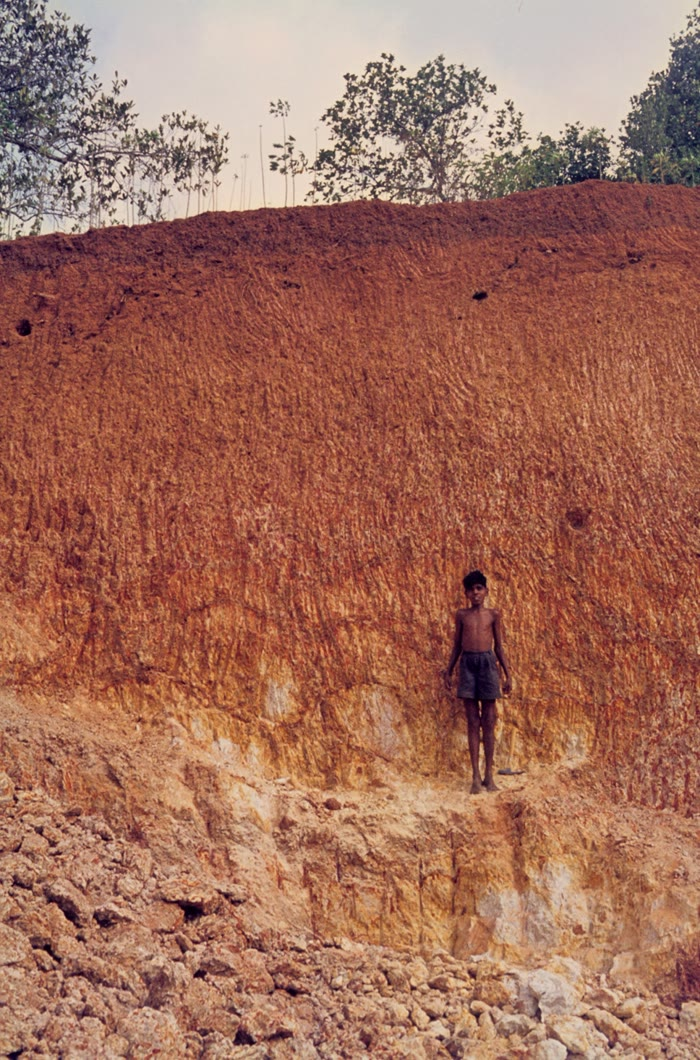
\includegraphics[height=8.5cm]{images/book2/g10-laterite-kerala.jpg}

{\small दक्षिणी भारत के केरल में ग्रेनाइटी नीस पर एक अपक्षय-प्रोफ़ाइल: नीचे
एक चितकबरी, अपघटित चट्टान; ऊपर, एक पतली मृदा के नीचे एक भूरी, हल्की-सी कठोर
\omterm{def:g10:soil-formation:laterite}{लैटेराइट}। लड़का पैमाना देता है। फ़ोटो: वर्नर
शेलमान, 1969 (CC~BY-SA~2.5)।}
\end{omfigure}

\begin{recall}
अपक्षय चट्टानों को उनके स्थान पर ही तोड़ता है; अपरदन टुकड़ों को दूर
ले जाता है; निक्षेपण उन्हें कहीं और जमा कर देता है (पुस्तक 1, कक्षा 5)। चट्टानें
खनिजों से बनी होती हैं, जैसे किसी ग्रेनाइट में क्वार्ट्ज़, फ़ेल्डस्पार और अभ्रक (पुस्तक 1, कक्षा
6)। मृदा खनिज कणों, ह्यूमस, जल, वायु और
जीवों की एक जीवित परत है; अपघटक मृत पदार्थ को ह्यूमस में बदलते हैं; किसी मृदा का वर्णन
उसकी परतों, या संस्तरों, से किया जाता है (जीव विज्ञान की पुस्तकें)। ऑक्सीकरण में कोई पदार्थ
इलेक्ट्रॉन खोता है, प्रायः ऑक्सीजन से संयोग करके (रसायन विज्ञान की पुस्तकें)।
\end{recall}

\section{चट्टान से मृदा तक}

भौतिक अपक्षय --- दरारों में पाले का जमना, गरम होना और ठंडा होना, जड़ें ---
चट्टान को उसके खनिज बदले बिना टुकड़ों में तोड़ता है। \omterm{def:g10:soil-formation:chemical-weathering}{रासायनिक अपक्षय}
स्वयं खनिजों को बदल देता है। दोनों मिलकर, लंबे समय में, ठोस चट्टान के ऊपरी भाग को
एक ढीले आवरण में बदल देते हैं, जो नीचे की ओर मोटा होता जाता है क्योंकि अपक्षय
नीचे की चट्टान को खाता जाता है।

\begin{definition}[जनक चट्टान; सैप्रोलाइट]\label{def:g10:soil-formation:weathering-profile}
किसी मृदा की \emph{जनक चट्टान}\index{जनक चट्टान} वह चट्टान है जिससे उसका
खनिज भाग बना। \emph{सैप्रोलाइट}\index{सैप्रोलाइट} अपक्षय द्वारा अपने स्थान पर ही
अपघटित चट्टान है: नरम और मिट्टी जैसी होते हुए भी वह जनक चट्टान के कण और
संरचना दिखाती है। \emph{अपक्षय-प्रोफ़ाइल} ताज़ी चट्टान से, सैप्रोलाइट
से होते हुए, शीर्ष की मृदा तक का पूरा स्तंभ है।
\end{definition}
% ledger: usgs:saprolite

\omterm{def:g10:soil-formation:weathering-profile}{सैप्रोलाइट} मोटी हो सकती है। संयुक्त राज्य अमेरिका के पूर्व में, ऐपलेशियन पर्वतों के
पूर्वी किनारे के अनुदिश लहरदार पहाड़ियों के नीचे, यह कहीं-कहीं लगभग
\qty{46}{m} (150 फ़ुट) तक पहुँचती है, यद्यपि इसकी मोटाई एक स्थान से दूसरे स्थान पर
बहुत बदलती है; मृदा उसका केवल ऊपरी भाग है।
% ledger: usgs:saprolite

\begin{omfigure}
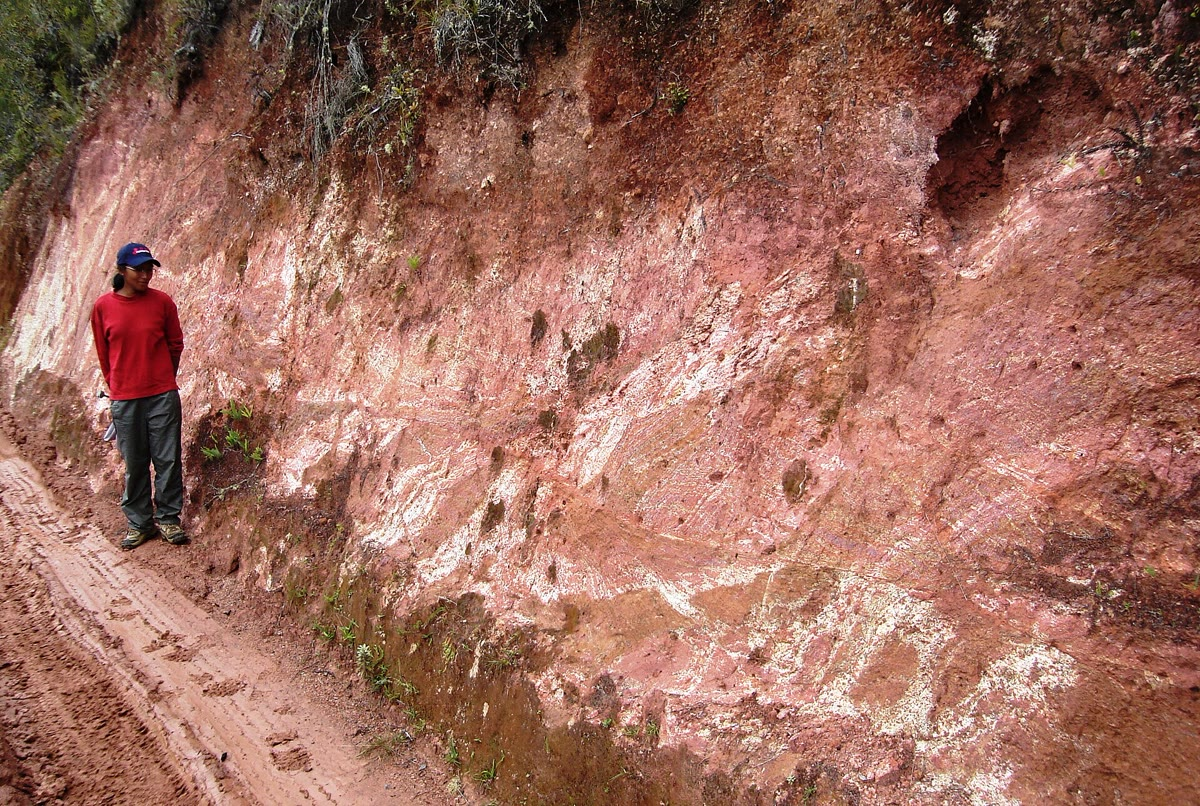
\includegraphics[width=0.8\linewidth]{images/book2/g10-saprolite-madagascar.jpg}

{\small मध्य मैडागास्कर में सड़क की एक कटाई में \omterm{def:g10:soil-formation:weathering-profile}{सैप्रोलाइट}: अपने स्थान पर ही अपघटित
पुरानी नीस अब भी अपनी पट्टियाँ लाल मिट्टी में सफ़ेद मृत्तिका की धारियों के रूप में
दिखाती है। फ़ोटो: डायोरिट (CC~BY-SA~3.0)।}
\end{omfigure}

\begin{omfigure}
\begin{tikzpicture}[font=\footnotesize]
  % humid tropical column
  \begin{scope}
    \fill[omThm!45!brown!60] (0,5.4) rectangle (1.8,6.0);
    \fill[omThm!70!orange!70] (0,4.2) rectangle (1.8,5.4);
    \fill[omThm!25!orange!35] (0,1.2) rectangle (1.8,4.2);
    \foreach \y in {1.5,2.1,2.7,3.3,3.9} \draw[white!80!black, thick] (0.1,\y) -- (1.7,\y+0.15);
    \fill[black!30] (0,0) rectangle (1.8,1.2);
    \foreach \x/\y in {0.3/0.3,0.9/0.7,1.4/0.2,0.5/0.9,1.2/1.0} \draw[black!55] (\x,\y) -- ++(0.2,0.08);
    \draw[black!60] (0,0) rectangle (1.8,6.0);
    \node[anchor=north, align=center] at (0.9,-0.1) {आर्द्र उष्णकटिबंध};
  \end{scope}
  % temperate column
  \begin{scope}[xshift=3.2cm]
    \fill[omThm!45!brown!60] (0,2.2) rectangle (1.8,2.6);
    \fill[omThm!25!orange!35] (0,1.2) rectangle (1.8,2.2);
    \foreach \y in {1.5,1.9} \draw[white!80!black, thick] (0.1,\y) -- (1.7,\y+0.15);
    \fill[black!30] (0,0) rectangle (1.8,1.2);
    \foreach \x/\y in {0.3/0.3,0.9/0.7,1.4/0.2,0.5/0.9,1.2/1.0} \draw[black!55] (\x,\y) -- ++(0.2,0.08);
    \draw[black!60] (0,0) rectangle (1.8,2.6);
    \node[anchor=north, align=center] at (0.9,-0.1) {शीतोष्ण\\जलवायु};
  \end{scope}
  % labels
  \draw[black!50] (5.3,5.7) -- (2.0,5.7); \node[anchor=west] at (5.4,5.7) {मृदा};
  \draw[black!50] (5.3,4.8) -- (2.0,4.8); \node[anchor=west, align=left] at (5.4,4.8) {लैटेराइट: लाल, लोहे और ऐलुमिनियम\\के ऑक्साइडों से समृद्ध};
  \draw[black!50] (5.3,3.4) -- (2.0,3.4); \node[anchor=west, align=left] at (5.4,3.4) {सैप्रोलाइट: अपने स्थान पर अपघटित\\चट्टान, संरचना बनी हुई};
  \draw[black!50] (5.3,0.6) -- (5.0,0.6); \node[anchor=west] at (5.4,0.6) {ताज़ी जनक चट्टान};
\end{tikzpicture}

{\small एक ही चट्टान पर दो अपक्षय-प्रोफ़ाइल (व्यवस्था-चित्र, पैमाने पर नहीं):
गरम, आर्द्र जलवायु में प्रोफ़ाइल कहीं अधिक मोटा होता है और उसका शीर्ष
\omterm{def:g10:soil-formation:laterite}{लैटेराइट} होता है; शीतोष्ण जलवायु में एक पतली \omterm{def:g10:soil-formation:weathering-profile}{सैप्रोलाइट} मृदा को धारण करती है।}
\end{omfigure}

\section{रासायनिक अपक्षय}

\begin{definition}[रासायनिक अपक्षय]\label{def:g10:soil-formation:chemical-weathering}
\emph{रासायनिक अपक्षय}\index{रासायनिक अपक्षय} जल के साथ और उसके द्वारा ले जाई
जाने वाली गैसों, कार्बन डाइऑक्साइड और ऑक्सीजन, के साथ अभिक्रियाओं द्वारा किसी चट्टान के खनिजों का
रूपांतरण है: कुछ खनिज घुल जाते हैं, कुछ नए खनिजों में बदल
जाते हैं, जो पृथ्वी की सतह पर स्थायी होते हैं।
\end{definition}

वर्षा का जल हवा से थोड़ी कार्बन डाइऑक्साइड घोलता है, और मृदा से रिसते हुए
उससे कहीं अधिक, जहाँ जड़ें और अपघटक इसे श्वसन में छोड़ते हैं। घुली हुई
गैस का एक भाग कार्बोनिक अम्ल बनाता है, जो हाइड्रोजन आयन मुक्त करता है:
\begin{center}
\ce{CO2 + H2O -> H+ + HCO3-}
\end{center}
ये हाइड्रोजन आयन खनिजों पर आक्रमण करते हैं।

\begin{definition}[जल-अपघटन]\label{def:g10:soil-formation:hydrolysis}
\emph{जल-अपघटन}\index{जल-अपघटन} जल और उसके हाइड्रोजन आयनों द्वारा किसी सिलिकेट
खनिज का \omterm{def:g10:soil-formation:chemical-weathering}{रासायनिक अपक्षय} है: हाइड्रोजन आयन खनिज के धातु आयनों का
स्थान ले लेते हैं, जो विलयन में चले जाते हैं, और खनिज का बाक़ी
भाग एक \omterm{def:g10:soil-formation:clay}{मृत्तिका खनिज} में पुनर्गठित हो जाता है।
\end{definition}

\begin{proposition}[फ़ेल्डस्पार का जल-अपघटन]\label{prop:g10:soil-formation:hydrolysis}
पोटैशियम फ़ेल्डस्पार ऑर्थोक्लेज़, \ce{KAlSi3O8}, \omterm{def:g10:soil-formation:hydrolysis}{जल-अपघटन} द्वारा
\omterm{def:g10:soil-formation:clay}{मृत्तिका खनिज} केओलिनाइट, \ce{Al2Si2O5(OH)4}, में बदल जाता है; पोटैशियम आयन और
घुली हुई सिलिका, \ce{H4SiO4}, जल द्वारा बहा ले जाए जाते हैं:
\begin{center}
\ce{2 KAlSi3O8 + 2 H+ + 9 H2O -> Al2Si2O5(OH)4 + 2 K+ + 4 H4SiO4}
\end{center}
\end{proposition}
% ledger: webmineral:formulas

\begin{proof}[जाँच]
दोनों पक्षों पर हर तत्त्व गिनिए। पोटैशियम: 2 और 2। ऐलुमिनियम: 2 और 2।
सिलिकॉन: 6 और $2 + 4 = 6$। ऑक्सीजन: $16 + 9 = 25$ और $9 + 16 = 25$।
हाइड्रोजन: $2 + 18 = 20$ और $4 + 16 = 20$। आवेश: $+2$ और $+2$।
\end{proof}

\begin{proposition}[कैल्साइट का विलयन]\label{prop:g10:soil-formation:calcite}
कैल्साइट, \ce{CaCO3}, यानी चूना पत्थर का खनिज, कार्बन डाइऑक्साइड वाले जल में
पूरी तरह घुल जाता है; कुछ भी ठोस नहीं बचता:
\begin{center}
\ce{CaCO3 + CO2 + H2O -> Ca^2+ + 2 HCO3-}
\end{center}
\end{proposition}
% ledger: webmineral:formulas

लोहे पर तीसरे ढंग से आक्रमण होता है। किसी चट्टान के गहरे रंग के खनिजों में, जैसे
किसी ग्रेनाइट का काला अभ्रक, लोहा अपचयित रूप \ce{Fe^2+} में होता है। जल द्वारा लाई गई
ऑक्सीजन इसका ऑक्सीकरण करती है, और लोहा(III) अविलेय
ऑक्साइडों के रूप में पीछे रह जाता है: पीला-भूरा गोएथाइट, \ce{FeO(OH)}, और लाल हेमेटाइट,
\ce{Fe2O3}। गोएथाइट के लिए:
\begin{center}
\ce{4 Fe^2+ + O2 + 6 H2O -> 4 FeO(OH) + 8 H+}
\end{center}
ये ऑक्साइड अपक्षयित चट्टानों और मृदाओं को पीला, भूरा और लाल रंग देते हैं।
% ledger: webmineral:formulas

सभी खनिज एक ही गति से अपक्षयित नहीं होते। अपक्षयित होते ग्रेनाइट में काला
अभ्रक ज़ंग खाता है और फ़ेल्डस्पार मृत्तिका बन जाते हैं, पर क्वार्ट्ज़ के कण, जो लगभग
अविलेय हैं, अपरिवर्तित निकल आते हैं: अंत में वे रेत बन जाते हैं।

\begin{example}[ग्रेनाइट का अपक्षय]\label{ex:g10:soil-formation:granite}
% ledger: webmineral:formulas (masses computed in figdata/grade-10/soil_rates.py)
एक किलोग्राम ऑर्थोक्लेज़ में $1000/278.33 \approx \qty{3.59}{mol}$
\ce{KAlSi3O8} होता है। समीकरण के अनुसार ऑर्थोक्लेज़ के दो मोल
केओलिनाइट का एक मोल देते हैं: $3.59/2 \approx \qty{1.80}{mol}$, यानी $1.80 \times 258.16
\approx \qty{464}{g}$ मृत्तिका। पोटैशियम, जो ऑर्थोक्लेज़ के द्रव्यमान का $14.05~\%$ है,
यानी \qty{140.5}{g}, और $2 \times 3.59 = \qty{7.19}{mol}$ सिलिका
विलयन में चले जाते हैं। क्वार्ट्ज़, फ़ेल्डस्पार और अभ्रक वाले ग्रेनाइट से अपक्षय
रेत (क्वार्ट्ज़), मृत्तिका (फ़ेल्डस्पार और अभ्रक से) और लोहे के ऑक्साइड छोड़ता है,
और पोटैशियम, सोडियम, कैल्शियम और सिलिका को नदियों में भेज देता है।
\end{example}

\section{मृत्तिका और ह्यूमस}

\begin{definition}[मृत्तिका खनिज]\label{def:g10:soil-formation:clay}
\emph{मृत्तिका खनिज}\index{मृत्तिका खनिज} परमाणुओं की एक-दूसरे पर रखी पतली
परतों से बना सिलिकेट है, जो अपक्षय से बनता है और रेत के कणों से कहीं छोटी
पपड़ियों के रूप में मिलता है। केओलिनाइट उनमें से एक है।
\end{definition}
% ledger: webmineral:formulas

मृत्तिका की पपड़ियों की सतहों पर ऋणात्मक विद्युत आवेश होते हैं। वे
धन आयनों --- पोटैशियम \ce{K+}, कैल्शियम \ce{Ca^2+}, मैग्नीशियम
\ce{Mg^2+}, अमोनियम \ce{NH4+} --- को थामे रखती हैं, जिन्हें अन्यथा
वर्षा बहा ले जाती। ह्यूमस भी यही करता है। आपस में बँधकर मृत्तिका और ह्यूमस
\emph{मृत्तिका--ह्यूमस संकुल} बनाते हैं, जो मृदा का खनिज पोषक तत्त्वों का भंडार है: एक जड़
हाइड्रोजन आयन छोड़ती है और बदले में पपड़ियों पर टिका पोटैशियम या कैल्शियम
ले लेती है।

\begin{omfigure}
\begin{tikzpicture}[font=\footnotesize, >={Stealth[length=2mm]}]
  \foreach \y in {0,0.7,1.4} {
    \fill[omExo!35, draw=black!60] (0,\y) rectangle (7.2,\y+0.3);
    \foreach \x in {0.3,0.9,...,7.0} \node[font=\tiny, black!70] at (\x,\y+0.15) {$-$};
  }
  \foreach \x/\ion in {0.7/K^+, 1.9/Ca^{2+}, 3.1/K^+, 4.3/Mg^{2+}, 5.5/NH_4^+, 6.7/K^+} {
    \fill[omThm!20, draw=omThm!80!black] (\x,2.1) circle (0.4);
    \node[font=\scriptsize] at (\x,2.1) {$\mathrm{\ion}$};
  }
  \foreach \x in {1.3, 3.7, 6.1} \fill[omThm!20, draw=omThm!80!black] (\x,0.5) circle (0.17);
  \foreach \x in {2.5, 4.9} \fill[omThm!20, draw=omThm!80!black] (\x,1.2) circle (0.17);
  \node[anchor=north] at (3.6,-0.1) {ऋणावेशित मृत्तिका-परतें, जिनके बीच धन आयन हैं};
  \node[anchor=south] at (3.1,2.5) {सतहों पर टिके धन आयन};
  % root and exchange
  \draw[line width=2.2pt, brown!60!black] (9.6,3.4) .. controls (9.3,2.6) and (8.9,2.2) .. (8.1,2.0);
  \node[anchor=east] at (9.25,3.3) {जड़};
  \draw[->, omDef!80!black, thick] (8.0,2.2) .. controls (7.6,2.6) and (7.2,2.6) .. (6.95,2.3);
  \node[anchor=south, omDef!80!black] at (7.5,2.55) {\ce{H+} दिया};
  \draw[->, omThm!80!black, thick] (6.95,1.8) .. controls (7.3,1.5) and (7.7,1.6) .. (8.0,1.85);
  \node[anchor=north, omThm!80!black] at (7.8,1.55) {\ce{K+} लिया};
\end{tikzpicture}

{\small मृत्तिका--ह्यूमस संकुल (व्यवस्था-चित्र): ऋणावेशित मृत्तिका-परतें
अपनी सतहों पर और अपने बीच धन आयनों को थामे रखती हैं; एक जड़ इन पोषक तत्त्वों के बदले
हाइड्रोजन आयन देती है।}
\end{omfigure}

\section{मृदा और जलवायु}

\omterm{def:g10:soil-formation:chemical-weathering}{रासायनिक अपक्षय} को जल चाहिए, और अधिकांश अभिक्रियाओं की तरह यह
गरमी में अधिक तेज़ चलता है। जहाँ जलवायु गरम और आर्द्र दोनों है, वहाँ चट्टान सबसे गहराई तक
और सबसे अधिक अपघटित होती है: फ़ेल्डस्पार पूरी तरह मृत्तिका बन जाते हैं, यहाँ तक कि सिलिका का भी अधिकांश भाग
बह जाता है, और जो बचता है वह सबसे कम विलेय तत्त्वों,
लोहे और ऐलुमिनियम, से समृद्ध होता है।

\begin{definition}[लैटेराइट]\label{def:g10:soil-formation:laterite}
\emph{लैटेराइट}\index{लैटेराइट} गरम, आर्द्र जलवायु का गहराई तक अपक्षयित पदार्थ है,
लाल या भूरा, जो मुख्यतः लोहे और ऐलुमिनियम के ऑक्साइडों और
केओलिनाइट से बना होता है, और जिससे लगभग सब कुछ विलेय हटाया जा चुका है।
\end{definition}

ठंडी जलवायु में, जो वर्ष के अधिकांश भाग जमी रहती है, और शुष्क जलवायु में,
जहाँ जल दुर्लभ है, \omterm{def:g10:soil-formation:chemical-weathering}{रासायनिक अपक्षय} धीमा होता है: मृदाएँ पतली होती हैं और
चट्टान ठीक नीचे होती है। ध्रुवों और भूमध्य रेखा के बीच अपक्षय की
गहराई आर्द्र उष्णकटिबंधीय वनों के नीचे सबसे अधिक और
मरुस्थलों तथा ध्रुवीय क्षेत्रों में सबसे कम होती है।

\begin{omfigure}
\begin{tikzpicture}[font=\footnotesize]
  \fill[black!25] (0,-0.2) -- (0,-0.5) .. controls (1.5,-0.6) and (2.5,-1.4) .. (3.4,-1.2)
     .. controls (4.2,-1.0) and (4.6,-0.55) .. (5.2,-0.5) .. controls (6.0,-0.5) and (6.6,-1.6) .. (7.6,-3.0)
     .. controls (8.2,-3.6) and (9.0,-3.6) .. (10,-3.4) -- (10,-3.8) -- (0,-3.8) -- cycle;
  \fill[omThm!25!orange!35] (0,0) -- (10,0) -- (10,-3.4) .. controls (9.0,-3.6) and (8.2,-3.6) .. (7.6,-3.0)
     .. controls (6.6,-1.6) and (6.0,-0.5) .. (5.2,-0.5) .. controls (4.6,-0.55) and (4.2,-1.0) .. (3.4,-1.2)
     .. controls (2.5,-1.4) and (1.5,-0.6) .. (0,-0.5) -- cycle;
  \draw[black!60] (0,0) -- (10,0);
  \node[anchor=south] at (0.6,0.05) {ध्रुवीय};
  \node[anchor=south] at (3.2,0.05) {शीतोष्ण};
  \node[anchor=south] at (5.3,0.05) {मरुस्थल};
  \node[anchor=south] at (6.8,0.05) {सवाना};
  \node[anchor=south] at (9.0,0.05) {उष्णकटिबंधीय वन};
  \node[anchor=north] at (0.4,-3.85) {ध्रुव};
  \node[anchor=north] at (9.6,-3.85) {भूमध्य रेखा};
  \node[black!70] at (2.0,-2.6) {ताज़ी चट्टान};
  \node[black!80] at (8.35,-1.0) {अपक्षयित चट्टान और मृदा};
\end{tikzpicture}

{\small ध्रुव से भूमध्य रेखा तक अपक्षय की गहराई (व्यवस्था-चित्र, गहराइयाँ
पैमाने पर नहीं): ध्रुवीय और मरुस्थली जलवायु में पतली, शीतोष्ण
जलवायु में मध्यम, आर्द्र उष्णकटिबंधीय वनों के नीचे सबसे अधिक।}
\end{omfigure}

\section{बनने में धीमी, खोने में तेज़}

मृदा कितनी तेज़ी से बनती है? मृदा-उत्पादन, यानी वह दर जिससे अपक्षय प्रोफ़ाइल के आधार पर
चट्टान को मृदा में बदलता है, संसार भर के अनेक स्थलों पर मापा गया है, और
वह दर भी जिससे सतह से मृदा का अपरदन होता है। इन मापनों का एक संकलन नीचे दी गई
प्रतिनिधि (माध्यिका) दरें देता है, हर एक प्रति वर्ष मृदा की मोटाई के रूप में व्यक्त।
% ledger: montgomery:rates

\begin{omfigure}
\begin{tikzpicture}
\begin{axis}[omrecord, width=0.82\linewidth, height=5.6cm, ymode=log, log origin=infty, ymin=0.005,
  ymax=5, ybar, bar width=16pt, xtick={0,1,2,3,4}, xmin=-0.6, xmax=4.6,
  xticklabels={{मृदा-\\उत्पादन}, {प्राकृतिक वनस्पति\\के नीचे अपरदन}, {भूवैज्ञानिक\\अपरदन}, {संरक्षण\\खेती}, {पारंपरिक\\जुताई}},
  xticklabel style={align=center, font=\scriptsize},
  ylabel={दर (\unit{mm} प्रति वर्ष)}, tick label style={font=\small}, label style={font=\small},
  nodes near coords, nodes near coords style={font=\scriptsize}, point meta=explicit symbolic]
\addplot[fill=omDef!45, draw=omDef!80!black] table[x=idx, y=rate_mm_yr, meta=rate_mm_yr] {figdata/out/grade-10-soil_rates-rates.dat};
\end{axis}
\end{tikzpicture}

{\small मापनों के एक वैश्विक संकलन से मृदा-उत्पादन और अपरदन की
माध्यिका दरें, मिलीमीटर मृदा प्रति वर्ष में (लघुगणकीय
पैमाना: हर चरण नीचे वाले का दस गुना है)। आँकड़े: मॉन्टगोमरी (2007),
\emph{PNAS} (अमेरिकी राष्ट्रीय विज्ञान अकादमी की शोध-पत्रिका)।}
\end{omfigure}
% ledger: montgomery:rates

प्राकृतिक वनस्पति के नीचे मृदा का अपरदन लगभग उतनी ही तेज़ी से होता है जितनी तेज़ी से वह बनती है,
लगभग \qty{0.02}{mm} प्रति वर्ष: लगभग छह शताब्दियों में एक सेंटीमीटर। पारंपरिक
जुताई में, जो फ़सलों के बीच ज़मीन को नंगा छोड़ देती है, अपरदन की माध्यिका दर
\qty{1.5}{mm} प्रति वर्ष है, मृदा-उत्पादन की दर का नब्बे गुना।
संरक्षण खेती में, जो मृदा को कम छेड़ती है और उसे ढका रखती है,
माध्यिका घटकर \qty{0.08}{mm} प्रति वर्ष रह जाती है, जो उत्पादन की दर के कहीं
अधिक निकट है।
% ledger: montgomery:rates (ratios computed in figdata/grade-10/soil_rates.py)

\begin{method}[बनने की दर की अपरदन की दर से तुलना]\label{met:g10:soil-formation:rates}
\begin{enumerate}
  \item दोनों दरों को एक ही इकाई (मिलीमीटर प्रति वर्ष) में व्यक्त कीजिए।
  \item शुद्ध हानि अपरदन की दर $E$ में से उत्पादन की दर $P$ घटाने पर मिलती है।
  \item मोटाई $S$ की मृदा $T = S/(E - P)$ वर्षों में खो जाती है; यदि
        $E \le P$, तो मृदा नहीं खो रही है।
  \item शून्य से मोटाई $S$ बनाने में $S/P$ वर्ष लगते हैं।
\end{enumerate}
\end{method}
% ledger: montgomery:lifetime

इन दरों के साथ एक मीटर मृदा को बनने में लगभग $1000/0.017 \approx 59\,000$
वर्ष लगते हैं, और पारंपरिक जुताई में यह लगभग
$1000/(1.537 - 0.017) \approx 660$ वर्षों में खो सकती है। मानवीय समय-पैमानों पर मृदा एक
ऐसा संसाधन है जिसका नवीकरण नहीं होता।
% ledger: montgomery:rates, montgomery:lifetime

\begin{omfigure}
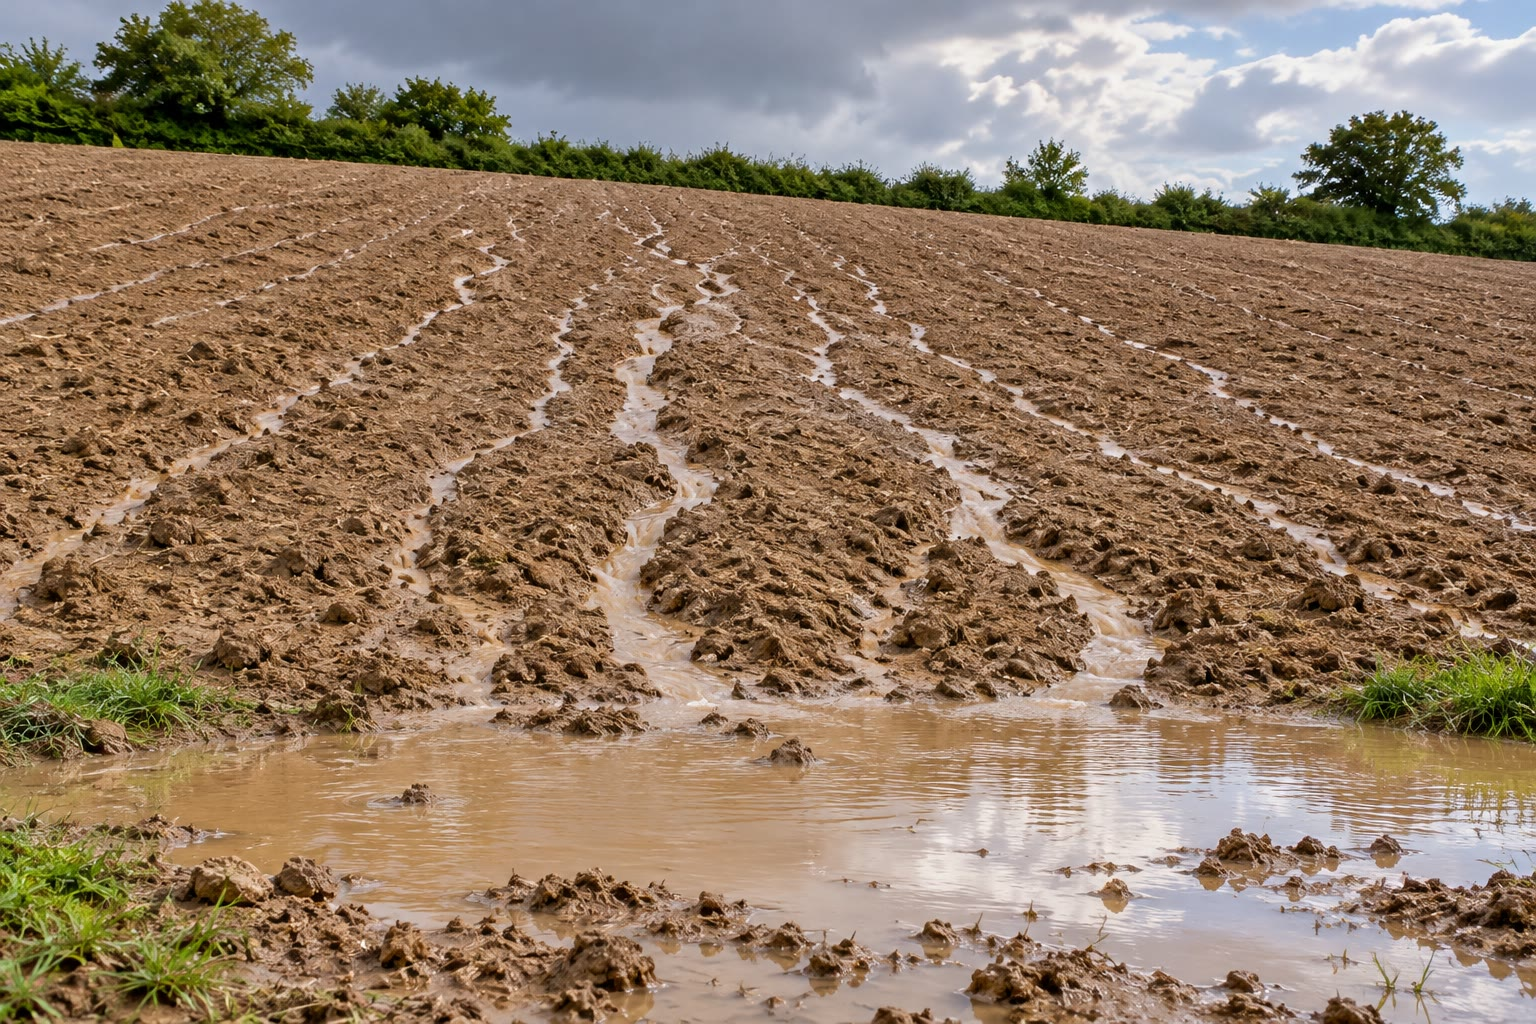
\includegraphics[width=0.72\linewidth]{images/book2/ai/g10-ploughed-rills.jpg}

{\small भारी तूफ़ान के बाद जुता हुआ एक खेत: अपवाह ने ढलान पर छोटी
नालियाँ, यानी क्षुद्र-सरिताएँ, काट दी हैं और मृदा को उसके तले के एक गंदले पोखर में
बहा ले गया है।}
\end{omfigure}

\section{अभ्यास}

\begin{exercise}[$\star$]\label{exo:g10:soil-formation:1}
\omterm{def:g10:soil-formation:chemical-weathering}{रासायनिक अपक्षय} और \omterm{def:g10:soil-formation:hydrolysis}{जल-अपघटन} की परिभाषा दीजिए।
\end{exercise}

\begin{exercise}[$\star$]\label{exo:g10:soil-formation:2}
\omterm{def:g10:soil-formation:weathering-profile}{सैप्रोलाइट} क्या है? आप \omterm{def:g10:soil-formation:weathering-profile}{सैप्रोलाइट} को नदी द्वारा लाई गई रेत में बनी मृदा से
कैसे अलग पहचान सकते हैं?
\end{exercise}

\begin{exercise}[$\star$]\label{exo:g10:soil-formation:3}
किसी ग्रेनाइट के अपक्षय के उत्पादों के नाम बताइए: उसके तीन मुख्य खनिजों में से हर एक
क्या बन जाता है?
\end{exercise}

\begin{exercise}[$\star$]\label{exo:g10:soil-formation:4}
अपक्षयित चट्टानें और उष्णकटिबंधीय मृदाएँ इतनी बार लाल, पीली या भूरी क्यों होती हैं?
\end{exercise}

\begin{exercise}[$\star$]\label{exo:g10:soil-formation:5}
दंड आरेख की सहायता से मृदा-उत्पादन की माध्यिका दर और पारंपरिक जुताई में अपरदन की
माध्यिका दर बताइए। दूसरी दर पहली से कितने गुना
बड़ी है?
\end{exercise}

\begin{exercise}[$\star\star$]\label{exo:g10:soil-formation:6}
जाँचिए कि कैल्साइट के विलयन का समीकरण हर तत्त्व के लिए और आवेश के लिए
संतुलित है।
\end{exercise}

\begin{exercise}[$\star\star$]\label{exo:g10:soil-formation:7}
चूना पत्थर पूरी तरह घुल जाता है, ग्रेनाइट रेत और मृत्तिका छोड़ता है। अध्याय की दो
अभिक्रियाओं की सहायता से यह अंतर समझाइए।
\end{exercise}

\begin{exercise}[$\star\star$]\label{exo:g10:soil-formation:8}
समझाइए कि मृत्तिका--ह्यूमस संकुल उस मृदा में पोटैशियम को कैसे बनाए रखता है जिसमें से वर्षा
बहकर निकलती है, और जड़ उसे कैसे लेती है।
\end{exercise}

\begin{exercise}[$\star\star$]\label{exo:g10:soil-formation:9}
\omterm{def:g10:soil-formation:laterite}{लैटेराइट} गरम, आर्द्र जलवायु में बनते हैं, ठंडी या शुष्क जलवायु में नहीं: इसके दो
कारण बताइए।
\end{exercise}

\begin{exercise}[$\star\star$]\label{exo:g10:soil-formation:10}
मृदा-उत्पादन की माध्यिका दर \qty{0.017}{mm} प्रति वर्ष है। \qty{1}{cm},
\qty{30}{cm} और \qty{1}{m} मृदा बनने में कितना समय लगता है?
\end{exercise}

\begin{exercise}[$\star\star$]\label{exo:g10:soil-formation:11}
अपरदन की दरें प्रायः प्रति हेक्टेयर प्रति वर्ष मृदा के द्रव्यमान के रूप में दी जाती हैं।
\qty{1200}{kg/m^3} के मृदा-घनत्व के साथ, प्रति वर्ष \qty{1.5}{mm} की हानि एक हेक्टेयर
(\qty{10000}{m^2}) पर कितना द्रव्यमान दर्शाती है?
\end{exercise}

\begin{exercise}[$\star\star\star$]\label{exo:g10:soil-formation:12}
किसी शीतोष्ण क्षेत्र की पहाड़ियों के नीचे \qty{46}{m} मोटी \omterm{def:g10:soil-formation:weathering-profile}{सैप्रोलाइट} बनी है।
यदि अपक्षय चट्टान में \qty{0.017}{mm} प्रति वर्ष की दर से आगे बढ़ा हो, तो इसमें कितना
समय लगा होगा? उत्तर ऐसे भूदृश्य की आयु के बारे में क्या संकेत
देता है?
\end{exercise}

\begin{exercise}[$\star\star\star$]\label{exo:g10:soil-formation:13}
अध्याय में दिया गया \ce{Fe^2+} के गोएथाइट में ऑक्सीकरण का समीकरण लिखिए
और उसकी जाँच कीजिए। फिर ऑक्सीजन और जल द्वारा \ce{Fe^2+} के
हेमेटाइट, \ce{Fe2O3}, में ऑक्सीकरण का समीकरण, \ce{H+} मुक्त करते हुए, लिखिए और संतुलित कीजिए।
\end{exercise}

\begin{exercise}[$\star\star\star$]\label{exo:g10:soil-formation:14}
संरक्षण खेती में अपरदन की माध्यिका दर \qty{0.082}{mm} प्रति
वर्ष है। \qty{0.017}{mm} प्रति वर्ष के मृदा-उत्पादन के साथ \qty{30}{cm} मृदा
खोने में कितना समय लगता है? पारंपरिक जुताई से तुलना कीजिए।
\end{exercise}

\begin{exercise}[$\star\star\star$]\label{exo:g10:soil-formation:15}
एक ग्रेनाइट में द्रव्यमान के अनुसार \qty{30}{\percent} ऑर्थोक्लेज़ है। जब इस ग्रेनाइट
के एक टन का सारा ऑर्थोक्लेज़ अपक्षयित हो चुका हो, तो कितना केओलिनाइट बनता है,
और कितना पोटैशियम मुक्त होता है?
\end{exercise}

\section{समस्या: एक मृदा का जीवनकाल}

\begin{problem}[{सप्ताहांत समस्या --- चट्टान से खेत तक और वापस नदी तक}]
\label{pb:g10:soil-formation:1}
% ledger: montgomery:rates, montgomery:lifetime, webmineral:formulas (values computed in figdata/grade-10/soil_rates.py)

\begin{center}
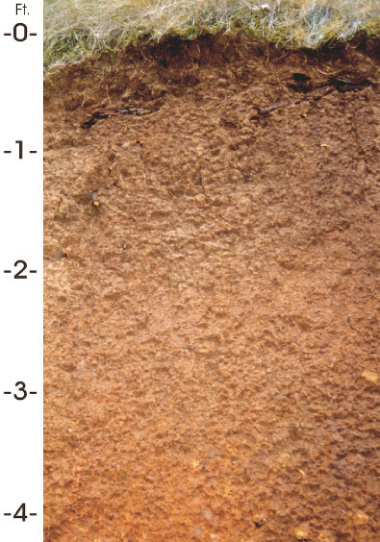
\includegraphics[height=6cm]{images/book2/g10-nrcs-jory-soil.jpg}

{\small बाईं ओर फ़ुट में पैमाने के साथ एक मृदा-प्रोफ़ाइल (\num{1}~फ़ुट =
\qty{0.3048}{m})। फ़ोटो: USDA प्राकृतिक संसाधन संरक्षण सेवा
(सार्वजनिक डोमेन)।}
\end{center}

\medskip
\noindent\textbf{भाग I --- एक प्रोफ़ाइल।}
\begin{enumerate}
  \item चित्र के तले के पास पैमाना 4 फ़ुट तक पहुँचता है। यह कितनी गहराई है,
        मीटर में?
  \item शीर्ष की गहरी परत लगभग आधा फ़ुट तक पहुँचती है। वह कितनी मोटी है,
        सेंटीमीटर में?
  \item इस शीर्ष परत को उसका गहरा रंग कौन देता है?
  \item नीचे मृदा लालिमा लिए भूरी है। कौन-से खनिज उसे यह
        रंग देते हैं, और वे कैसे बने?
  \item क्या फ़ोटो में \omterm{def:g10:soil-formation:weathering-profile}{जनक चट्टान} दिखाई देती है? चित्र के तले के नीचे आप क्या
        मिलने की अपेक्षा करेंगे?
\end{enumerate}

\medskip
\noindent\textbf{भाग II --- अपक्षयित होते ग्रेनाइट का रसायन।}
\begin{enumerate}[resume]
  \item ऑर्थोक्लेज़ के \omterm{def:g10:soil-formation:hydrolysis}{जल-अपघटन} का समीकरण लिखिए।
  \item \qty{1}{kg} में ऑर्थोक्लेज़ के कितने मोल हैं
        (\qty{278.33}{g/mol})?
  \item वे कितना केओलिनाइट (\qty{258.16}{g/mol}) देते हैं?
  \item जल में क्या निकल जाता है, और वह कहाँ जाता है?
  \item ग्रेनाइट के क्वार्ट्ज़ का क्या होता है?
\end{enumerate}

\medskip
\noindent\textbf{भाग III --- बनना बनाम अपरदन।}
\begin{enumerate}[resume]
  \item मृदा \qty{0.017}{mm} प्रति वर्ष की दर से बनती है। भाग I का प्रोफ़ाइल
        बनने में कितना समय लगता है?
  \item पारंपरिक जुताई में मृदा का अपरदन \qty{1.537}{mm} प्रति
        वर्ष होता है। हर वर्ष शुद्ध हानि कितनी है?
  \item भाग I का प्रोफ़ाइल कितने समय तक टिकेगा?
  \item प्रश्न 11 और 13 के दोनों समयों की तुलना कीजिए।
  \item प्राकृतिक वनस्पति के नीचे अपरदन \qty{0.013}{mm} प्रति वर्ष है। क्या
        मृदा खो रही है?
\end{enumerate}

\medskip
\noindent\textbf{भाग IV --- मृदा का जीवनकाल।}
\begin{enumerate}[resume]
  \item समय $T$ को, जो मोटाई $S$ की मृदा खोने में लगता है,
        $S$, अपरदन की दर $E$ और उत्पादन की दर $P$ के फलन के रूप में लिखिए।
  \item $T$ परिकलित कीजिए, पारंपरिक जुताई में $S = \qty{30}{cm}$ के लिए।
  \item $T$ परिकलित कीजिए, संरक्षण खेती में $S = \qty{30}{cm}$ के लिए
        (\qty{0.082}{mm} प्रति वर्ष)।
  \item मृदा को ऐसा संसाधन क्यों कहा जा सकता है जिसका मानवीय
        समय-पैमानों पर नवीकरण नहीं होता?
  \item पारंपरिक जुताई में एक मीटर मृदा खोने में कितना समय लगता है?
\end{enumerate}
\end{problem}
